\subsection{The Galaxy Stellar Mass Function}
\label{sec:results:gsmf}

The Galaxy Stellar Mass Function (GSMF) describes the number of galaxies per unit volume per unit stellar mass interval d$\log_{10}M$,
\begin{align}
    \phi(M) = N \,/\, \mathrm{Mpc^{-3} \, dex^{-1}}\;\;,
\end{align}
and is commonly described using a Schechter function \citep{schechter_analytic_1976},
\begin{align}
  \phi(M) \, \mathrm{d}\log_{10}M = \mathrm{ln}(10) \, \phi^* \, e^{-M/M^*} \, \left(\frac{M}{M^*} \right)^{\alpha + 1},
\end{align}
which describes the high- and low-mass behaviour with an exponential and a power law dependence on stellar mass, respectively.
Recent studies have found that a double Schechter function can better fit the full distribution \citep[\textit{e.g.} the GAMA survey, ][]{baldry_galaxy_2008}.
\begin{align}
    \phi(M) \, \mathrm{d}\log_{10}M& = \mathrm{ln}(10) \, e^{-M/M^*} \times \nonumber\\
    & \left[ \, \phi^{*}_{1} \, \left(\frac{M}{M^*} \right)^{\alpha_{1} + 1} + \phi^{*}_{2} \, \left( \frac{M}{M^*} \right)^{\alpha_{2} + 1} \right].
\end{align}
The slope of the shallower power-law component is not well-constrained by the data and so we fix it at $\alpha_2=-1$.
We define the stellar mass $M_{*}$ as the total mass of all star particles within a 30 kpc aperture centred on the potential minimum of the subhalo.

\subsubsection{The cosmic GSMF}
\label{sec:cos_gsmf}

In this section, we present results for the universal GSMF, averaged within our (3.2\,cGpc)$^3$ box.  This is obtained by combining the individual GSMFs from each of our resimulation volumes with appropriate weighting, as described in \Sec{method:weighting}.

\begin{figure}
	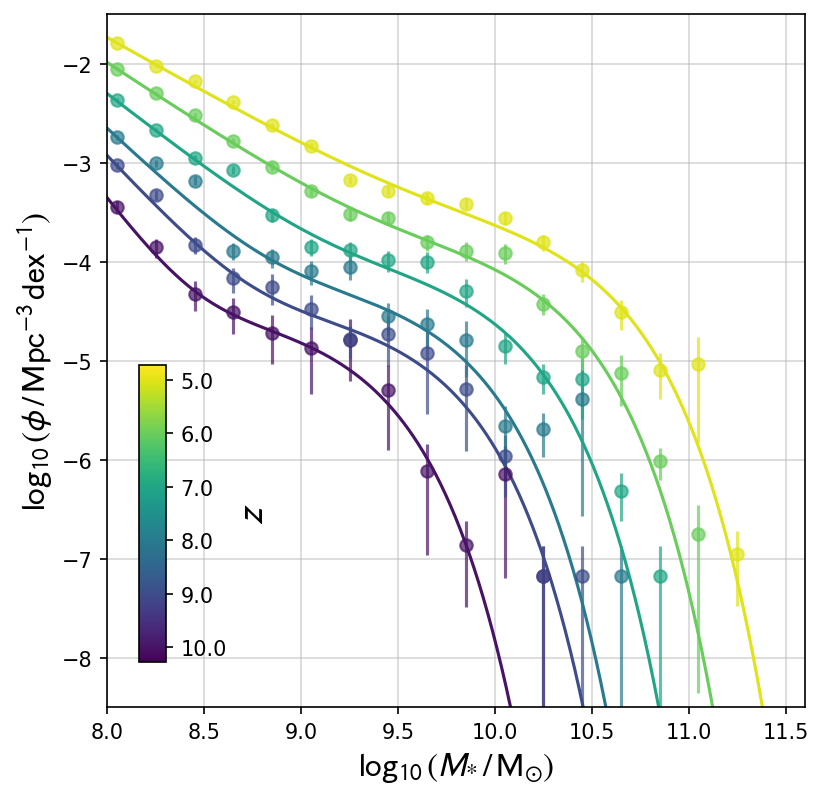
\includegraphics[width=\columnwidth]{images/gsmf_all.png}
  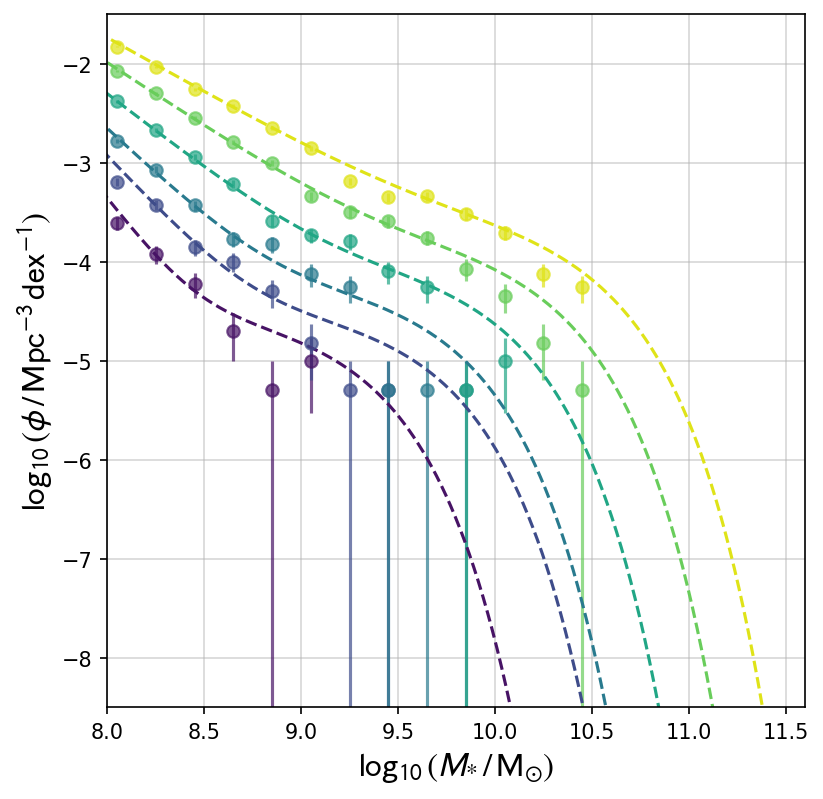
\includegraphics[width=\columnwidth]{images/gsmf_all_ref.png}
    \caption{\textit{Top:} Redshift evolution of the \flares\ composite galaxy stellar mass function.
    Points show binned differential counts with Poisson $1\sigma$ uncertainties from the simulated number counts.
    Solid lines show double-Schechter function fits, quoted in \tab{schechter_params}. The parameter evolution is shown in \fig{fit_param_evolution}.
    \textit{Bottom:} as for the top panel, but points show the counts from the periodic Reference volume. The dashed lines show the double-Schechter fitted relation from \flares. The coverage of the massive end in the periodic volume is poor.
    }
    \label{fig:gsmf}
\end{figure}

\begin{figure}
	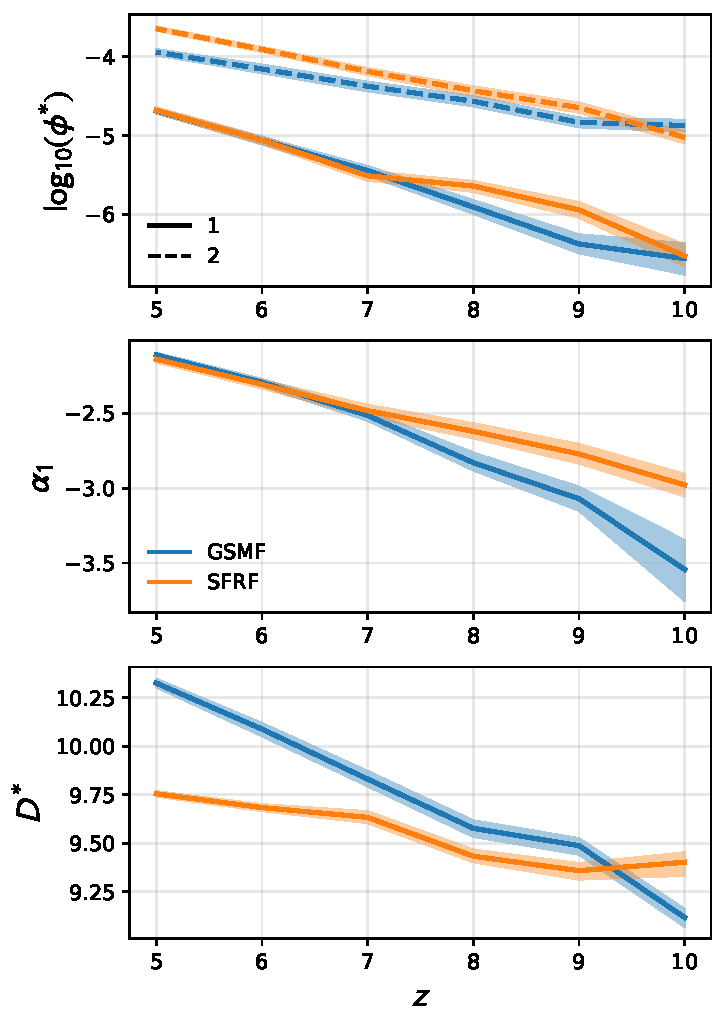
\includegraphics[width=\columnwidth]{images/fit_param_evolution.pdf}
    \caption{Parameter evolution for double-Schechter function fits to the \flares\ composite galaxy stellar mass function (GSMF, circles) and star formation rate function (SFRF, diamonds).
    The low (A) and high (B) mass components are shown with filled and hollow points, respectively.
    The low-mass slope of the high-mass component ($\alpha_{2}$) is fixed at -1.
    The characteristic mass of the GSMF ($\mathrm{M_{*}}$) and the characteristic SFR of the SFRF ($\SFR_*$) are shown in the bottom panel, labelled $D_*$.
    $\SFR_*$ is offset by $+10^{8}$ to aid comparison with $M_{*}$.
    The GSMF and SFRF show very similar behaviour; the normalisation of both components and the low-mass slope all increase with decreasing redshift.
    The characteristic mass increases with decreasing redshift for the GSMF, whereas the characteristic star formation rate of the SFRF shows a flatter redshift relation.
    }
    \label{fig:fit_param_evolution}
\end{figure}

The top panel of \fig{gsmf} shows the GSMF for redshifts between $z = 5 \mapsto 10$.
We show differential counts in bins $0.2 \, \mathrm{dex}$ in width (with 1$\sigma$ uncertainties).
The solid lines show double-Schechter function fits at each integer redshift.
The normalisation increases with decreasing redshift, and the characteristic mass (or knee) of the distribution shifts to higher masses.
This is more clearly seen in \fig{fit_param_evolution}, which shows the evolution of the double-Schechter parameters with redshift.
The low-mass slope also gets shallower with decreasing redshift, from $-3.5$ at $z = 10$ to $-2.0$ at $z = 5$.



% \begin{figure}
% 	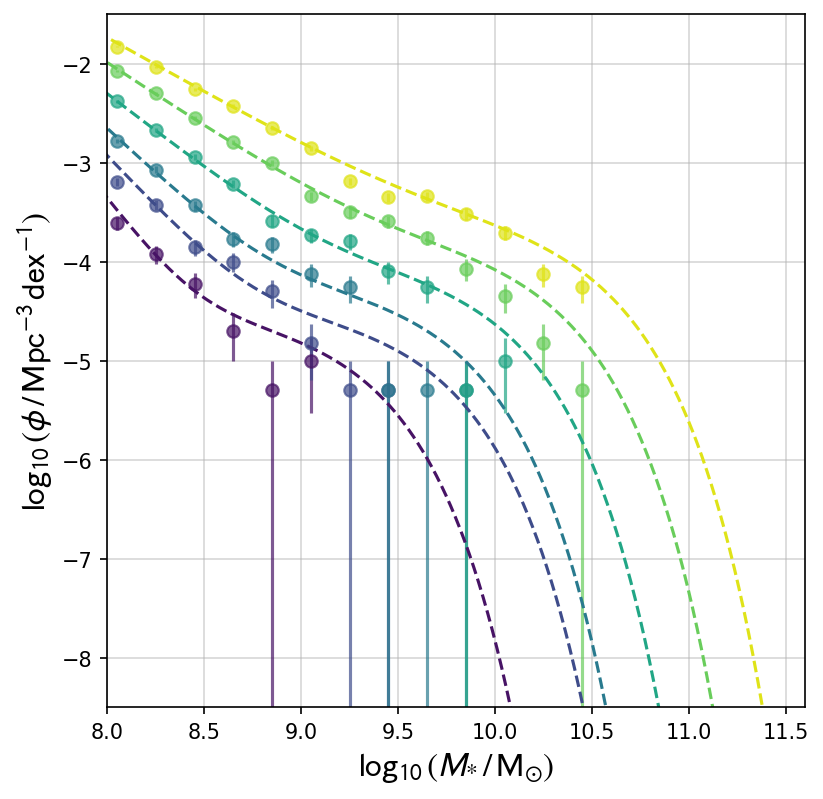
\includegraphics[width=\columnwidth]{images/gsmf_all_ref.png}
%     \caption{Redshift evolution of the periodic Reference volume galaxy stellar mass function. Points show binned differential counts, with 1$\sigma$ uncertainties. Dashed lines show the double-Schechter fits to the \flares\ composite GSMF shown in \fig{gsmf}.
%     }
%     \label{fig:gsmf_ref}
% \end{figure}

Our composite GSMF significantly extends the dynamic range of the GSMF compared to the periodic volumes.
To demonstrate, the bottom panel of \fig{gsmf} shows the \flares\ double-Schechter fits, alongside the binned counts from the Reference periodic volume.
At each redshift the maximum stellar mass probed is approximately an order of magnitude larger in \flares.
In fact, the periodic reference volume barely probes the exponential tail of the high mass component of the GSMF.
When fitting a double-Schechter to the binned Reference volume counts we found that the parameters of the high mass component were completely unconstrained.
However, it is clear from the bottom panel of \fig{gsmf} that the low-mass slope is consistent between the Reference volume and \flares.
We have also tested that this is the case for the $(50 \; \mathrm{Mpc})^{3}$ AGNdT9 periodic volume.


\begin{figure*}
	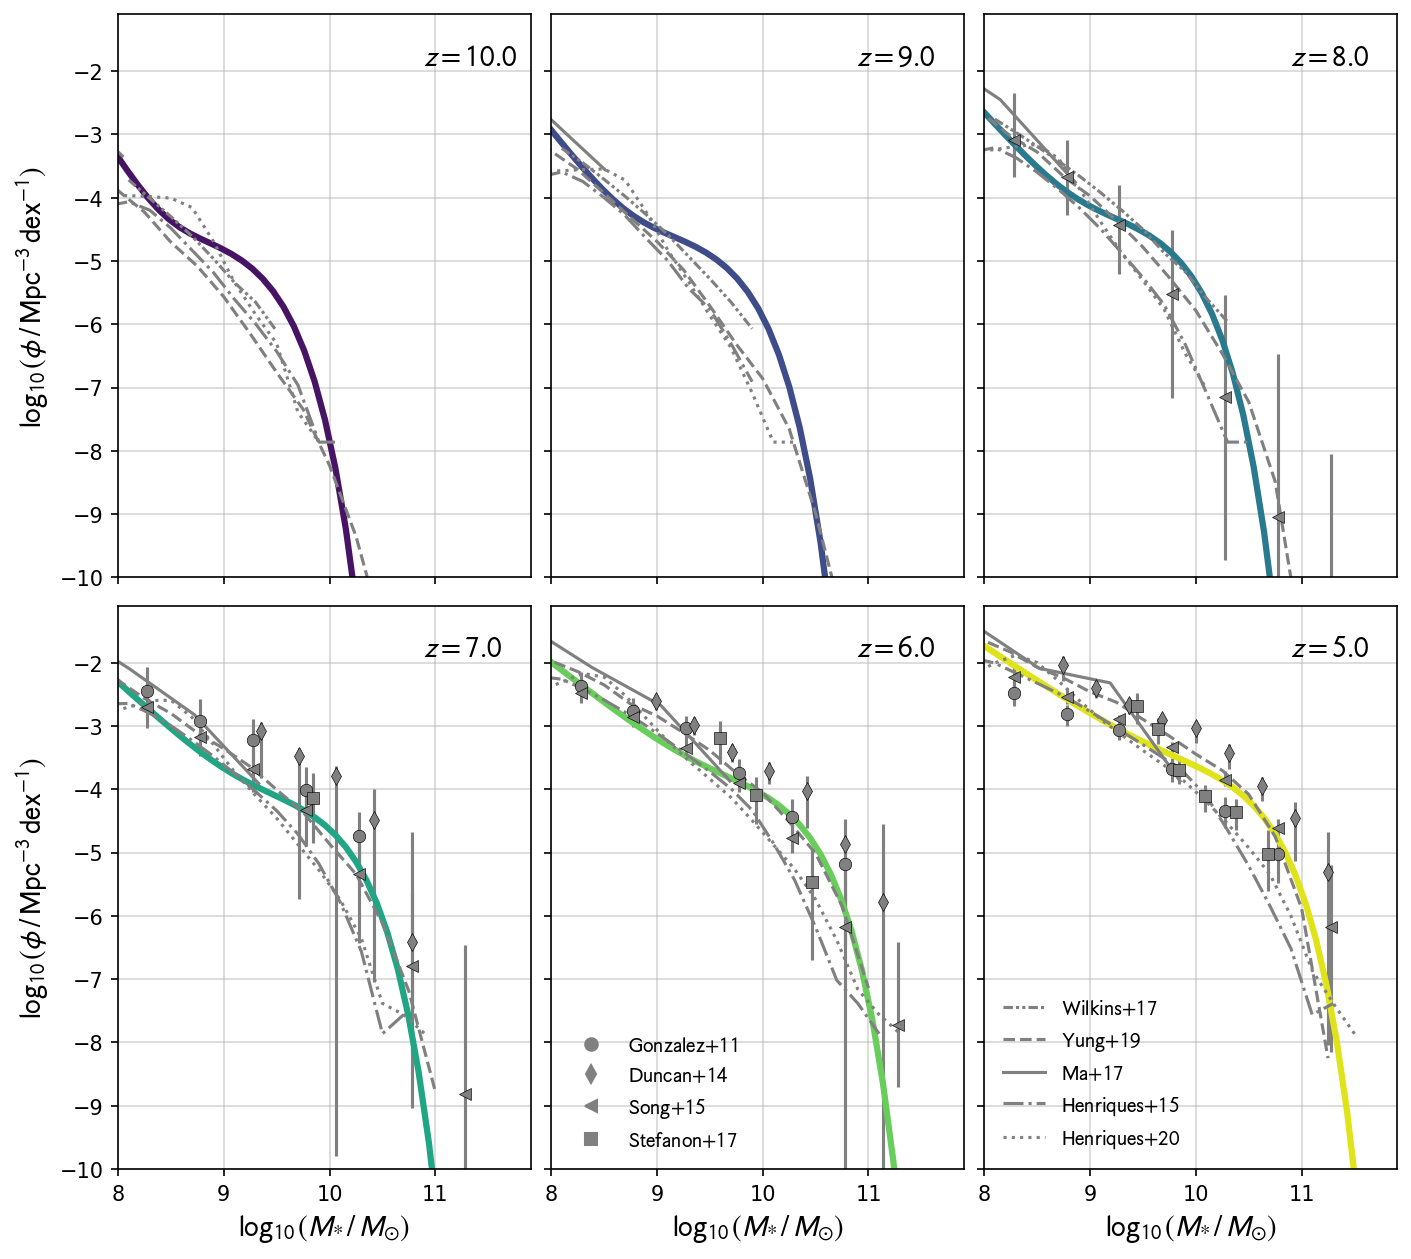
\includegraphics[width=\textwidth]{images/gsmf_multi_both.png}
    \caption{\flares\ composite galaxy stellar mass function evolution, alongside observational constraints \citep{gonzalez_evolution_2011,duncan_mass_2014,song_evolution_2016,stefanon_rest-frame_2017} as well as predictions from other models \citep{yung_semi-analytic_2019,ma_simulating_2018,henriques_galaxy_2015,henriques_l-galaxies_2020}.
    There is some disagreement over the normalisation of the GSMF between different observational studies, however \flares\ is consistent up to $z = 7$.
    }
    \label{fig:gsmf_multi_both}
\end{figure*}

In \fig{gsmf_multi_both} we show the composite \flares\ GSMF against a number of high-$z$ observational constraints in the literature \citep{gonzalez_evolution_2011,duncan_mass_2014,song_evolution_2016,stefanon_rest-frame_2017}.
These studies show a spread of $\sim 0.5 \; \mathrm{dex}$ at $z = 5$, which highlights the difficulty of accurately measuring the GSMF at high redshift.
The \flares\ composite GSMF lies within this inter-study scatter, most closely following the relations derived by \cite{song_evolution_2016} up to $z = 7$.
There are few observational constraints at $z \geqslant 8$, but where they exist \flares\ is within the (large) uncertainties at all masses.


We also compare in \fig{gsmf_multi_both} to predictions from other galaxy formation models.
The Feedback In Realistic Environments (\textsc{Fire}) project performed zoom simulations of individual halos with masses between $10^{8} \;-\; 10^{12} \, M_{\odot}$, which were then combined to provide a composite galaxy stellar mass function probing the low-mass regime \citep{ma_simulating_2018}.
\flares\ is consistent with \textsc{Fire} at all redshifts where their mass range overlaps.
\fig{gsmf_multi_both} also shows both the 2015 and 2020 versions of \lgals.
Both models are in reasonably good agreement at all redshifts shown, but tend to underestimate the number density of massive galaxies at $z=5$ compared to both \flares\ and the observations.

\cite{yung_semi-analytic_2019} presented results from the Santa Cruz semi-analytic model \citep{somerville_star_2015}, which extends to a wide dynamic range.
Whilst \flares\ is consistent with this model for $z \leqslant 7$, at $z \geqslant 8$ the Santa Cruz model predicts a more power-law shape to the GSMF, with a lower normalisation at the characteristic mass.
This is in agreement with the observed flattening of the GSMF with increasing redshift.


\subsubsection{Environmental dependence of the GSMF}
\label{sec:env_gsmf}

\begin{figure}
	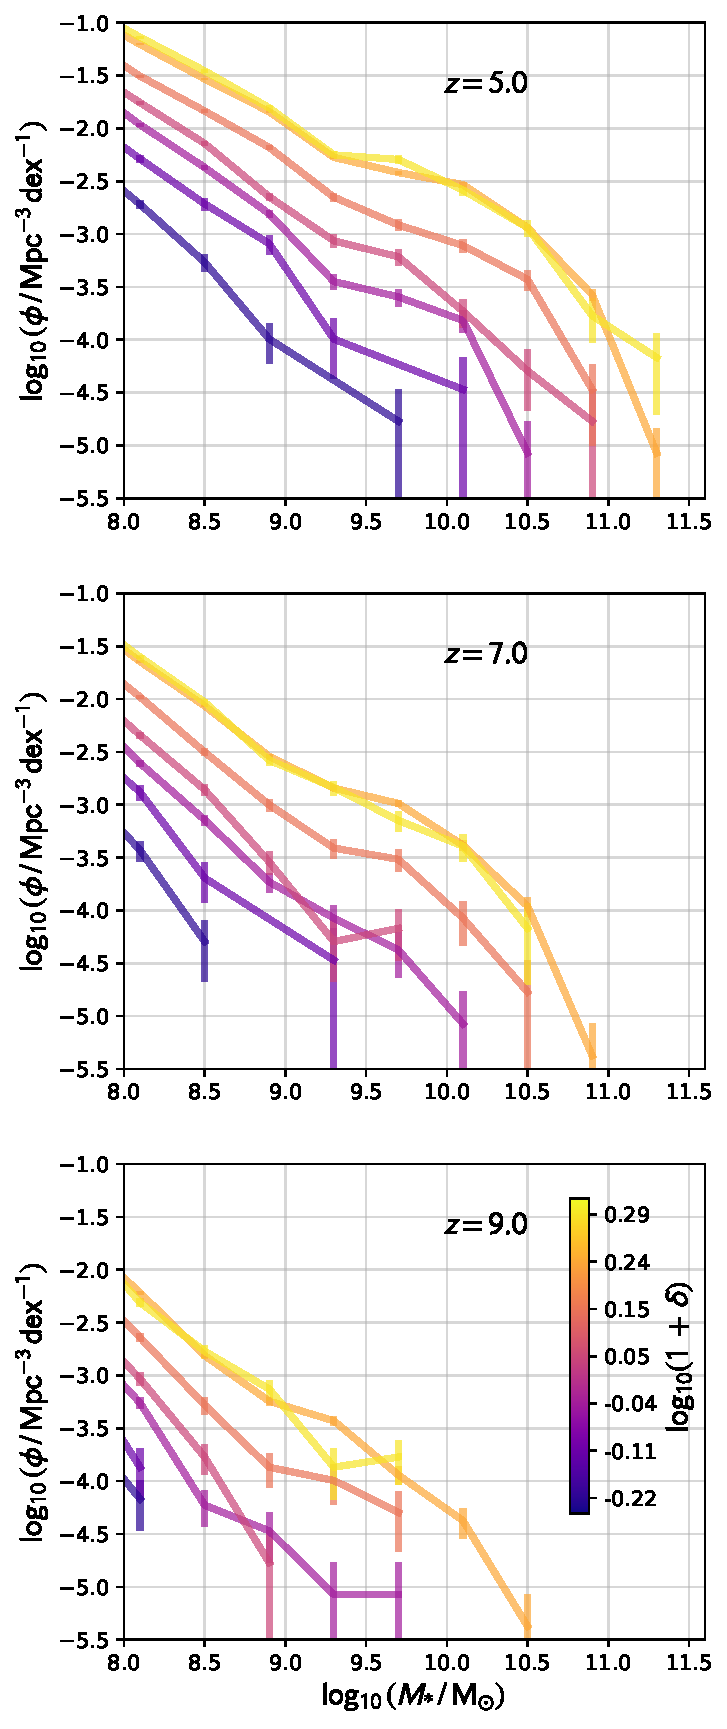
\includegraphics[width=\columnwidth]{images/gsmf_overdensity.pdf}
    \caption{The \flares\ GSMF between $z = 5$ and $9$ split by binned log-overdensity.
    Poisson 1$\sigma$ uncertainties are shown for each bin from the simulated number counts.
    The normalisation increases with increasing overdensity, and probes higher stellar masses.}
    \label{fig:gsmf_overdensity}
\end{figure}

Our zoom simulations of a range of overdensities not only allow us to construct a composite GSMF for the entire $(3.2 \, \mathrm{Gpc})^{3}$ volume, but also investigate the environmental effect on the GSMF.
\sec{method} demonstrates the wide range of environments probed, from extremely underdense void regions, to the most overdense high redshift structures that are likely to collapse in to massive, $> 10^{15} \; \mathrm{M_{\odot}}$ clusters by $z = 0$ \citep{chiang_ancient_2013,lovell_characterising_2018}.

\fig{gsmf_overdensity} shows the GSMF in bins of log-overdensity from $z = 5 - 9$.
We use wider bins than previously ($0.4 \, \mathrm{dex}$) due to the lower galaxy numbers in each re-simulation.
As expected, higher overdensity regions have a higher normalisation, $\sim +2 \; \mathrm{dex}$ above the lowest overdensity regions at $\mathrm{M_{*}} \,/ \mathrm{M_{\odot}} = 10^{9.5} \; (z = 5)$.
There is also an apparent difference in the shape as a function of log-overdensity:
lower overdensity regions exhibit a distribution that is more power-law -like, whereas higher overdensity regions clearly show a double-Schechter -like knee.
This may be due to the higher number of galaxies in the overdense regions, better sampling the knee, but may also point to differing assembly histories for galaxies in different environments.
We will explore the star formation and assembly histories more closely in future work.


The dependence of the GSMF on overdensity may explain the tension between the composite \flares\ GSMF and other models at $z > 7$ seen in \fig{gsmf_multi_both}.
Our much larger box allows us to sample extreme overdensities that are not present in smaller volumes.
Observationally, the \cite{song_evolution_2016} results show a more power law-like form at $z = 8$.
Double-schechter forms of the GSMF at low-$z$ have been attributed to the contribution of a passive and star forming population, each fit individually by a single schechter function \citep{kelvin_galaxy_2014,moffett_galaxy_2016}, though this separation is not perfect \citep[\textit{e.g.}][]{ilbert_mass_2013,tomczak_sfr-m*_2016}.
The robust double-schechter shape measured in \flares\ at $z \geqslant 8$ is therefore curious; we see in \app{ssfr_cut} that there is no significant passive population as a function of stellar mass.
We therefore tentatively suggest that the tension may be due to the small volume probed observationally at these depths, which does not probe extreme environments that contribute significantly to the cosmic GSMF.


We do not fit each binned GSMF in log-overdensity as there are insufficient galaxies to provide a robust fit.
However, we do provide fits to the normalisation at a given stellar mass and redshift, in the following form,
\begin{equation}
  \phi \,(\mathrm{log_{10}}(1+\delta) \,|\, M_{*}, z) = m \,[\mathrm{log_{10}}(1+\delta)] + c,
\end{equation}
where $\mathrm{log_{10}}(1\,+\,\delta)$ is the overdensity of the region.
\tab{norm_GSMF} shows these fits for bins $\pm 0.2$ dex wide centred at $\mathrm{log_{10}(M_{*}/M_{\odot})} = [8.5,\,9.7]$.
% \peter{I do not understand what this means, or what is being fit.  Is it s restricted range in mass?}
% \peter{Why are we bothering with these fits anyway?  We don't use them in this paper and I can't think of any reason why other people might quote them.}

\begin{table}
	\centering
	\caption{Fits to the normalisation, $\log_{10}(\phi/$Mpc$^{-3}$dex$^{-1}$), of the GSMF at different redshifts and masses (see \sec{env_gsmf}).}
	\label{tab:norm_GSMF}
	\begin{tabular}{cccc} % four columns, alignment for each
		\hline
		$z$ & $\mathrm{log_{10}(M_{*}/M_{\odot})}$ & $m$ & $c$ \\
		\hline
        5 & 8.5 & 3.5 & -2.4 \\
        7 & 8.5 & 4.4 & -3.2 \\
        9 & 8.5 & 4.6 & -4.0 \\
        5 & 9.7 & 4.8 & -3.6 \\
        7 & 9.7 & 4.4 & -4.2 \\
        9 & 9.7 & 4.0 & -4.9 \\
    \hline
	\end{tabular}
\end{table}


% \begin{align}
%     \phi(M) \, \mathrm{d}M = \mathrm{exp}\left( \frac{-M}{M_{*}} \right) \left[ \phi_{*,1} \, \left( \frac{M}{M_{*}}\right)^{\alpha_1} + \phi_{*,2} \, \left( \frac{M}{M_{*}}\right)^{\alpha_2} \right] \frac{\mathrm{d}M}{M_{*}}\;\;,
% \end{align}


% \todo{add random errors and measure effect on high-mass end (see Furlong+15, 3.2.1)}
